\documentclass{beamer}
\usepackage{booktabs} % Allows the use of \toprule, \midrule and \bottomrule for better rules in tables
\usepackage[T1]{polski}
\usepackage{graphicx}
\usepackage{caption}
\usepackage{amsmath}
\usepackage{amsthm}
\usepackage{palatino}
\usepackage{helvet}
\graphicspath{{images/}{./}}
\newcommand{\modulo}[1]{\mathbb{Z}_{#1}}
\usetheme{Madrid}
\usefonttheme{default}
\useinnertheme{circles}
\setbeamertemplate{frametitle}[default][center]
%Information to be included in the title page:
\title[Symulator phyether]{\textbf{Dydaktyczny symulator wybranych rozwiązań warstwy fizycznej sieci Ethernet}}
\author[Iwanicki M., Bauer M., Garnowski M.]{Michał Iwanicki, Mateusz Bauer, Marcin Garnowski}
\institute[PG]{Politechnika Gdańska}
\date{\today}

\begin{document}

\frame{\titlepage}

\begin{frame}
    \frametitle{Uruchamianie}
    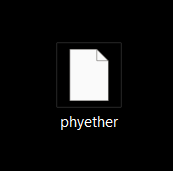
\includegraphics[width=0.25\textwidth]{prezentacja_start1.png}
    \hfill
    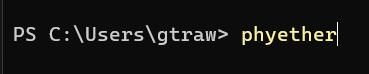
\includegraphics[width=0.65\textwidth]{prezentacja_start2.png}
\end{frame}

\begin{frame}
    \frametitle{Poruszanie się po symulatorze}
    \begin{center}
        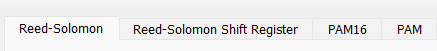
\includegraphics[width=0.95\textwidth]{zakladki.png}
    \end{center}
\end{frame}

\begin{frame}
    \frametitle{Reed-Solomon}
    \begin{center}
        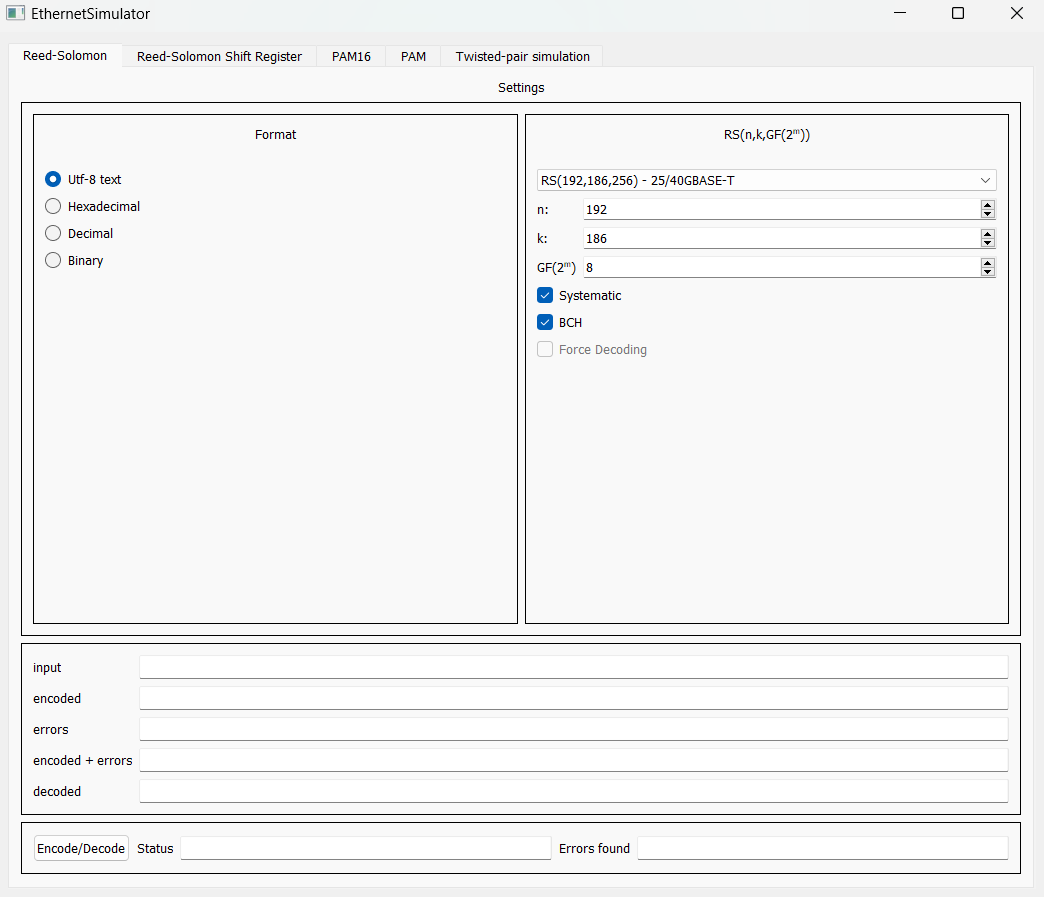
\includegraphics[width=0.95\textwidth,height=0.85\textheight,keepaspectratio]{prezentacja_rs.png}
    \end{center}
\end{frame}

\begin{frame}
    \frametitle{Reed-Solomon Shift Register}
    \begin{center}
        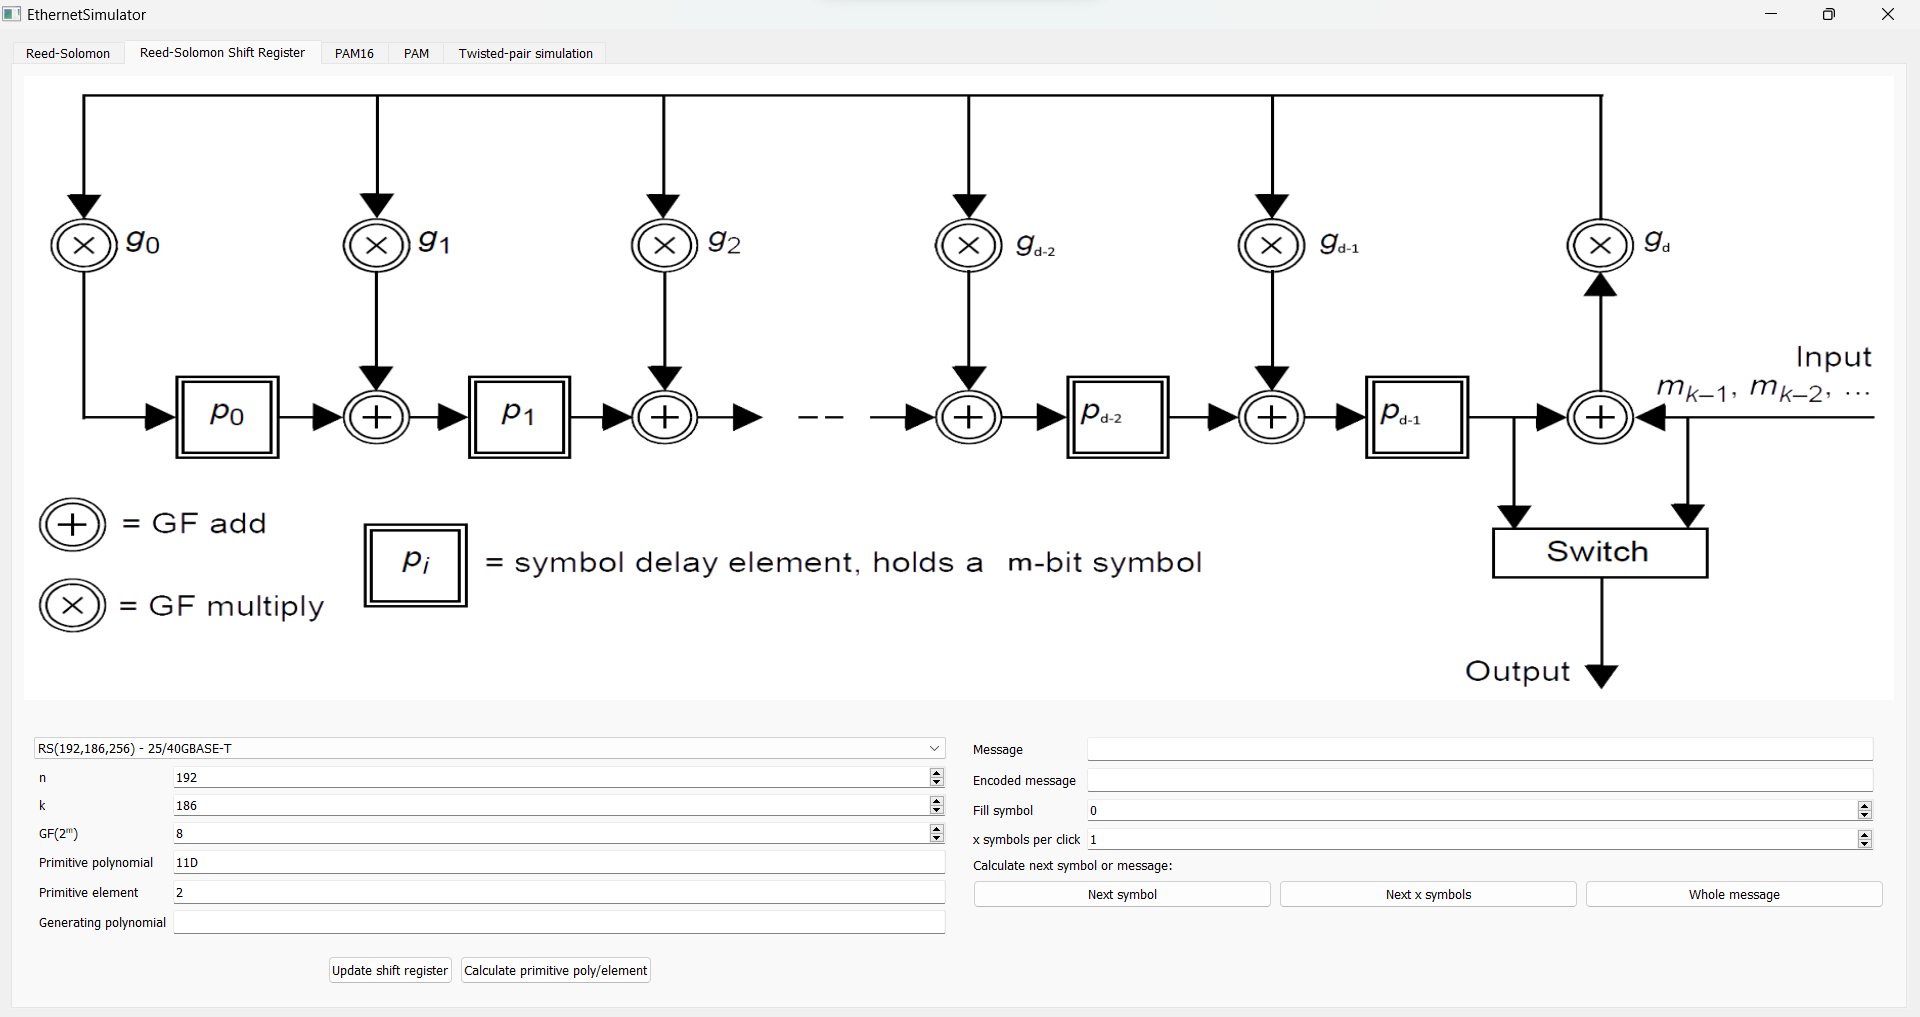
\includegraphics[width=0.95\textwidth, height=0.85\textheight,keepaspectratio]{prezentacja_rs_sr.png}
    \end{center}
\end{frame}

\begin{frame}
    \frametitle{PAM16}
    \begin{center}
        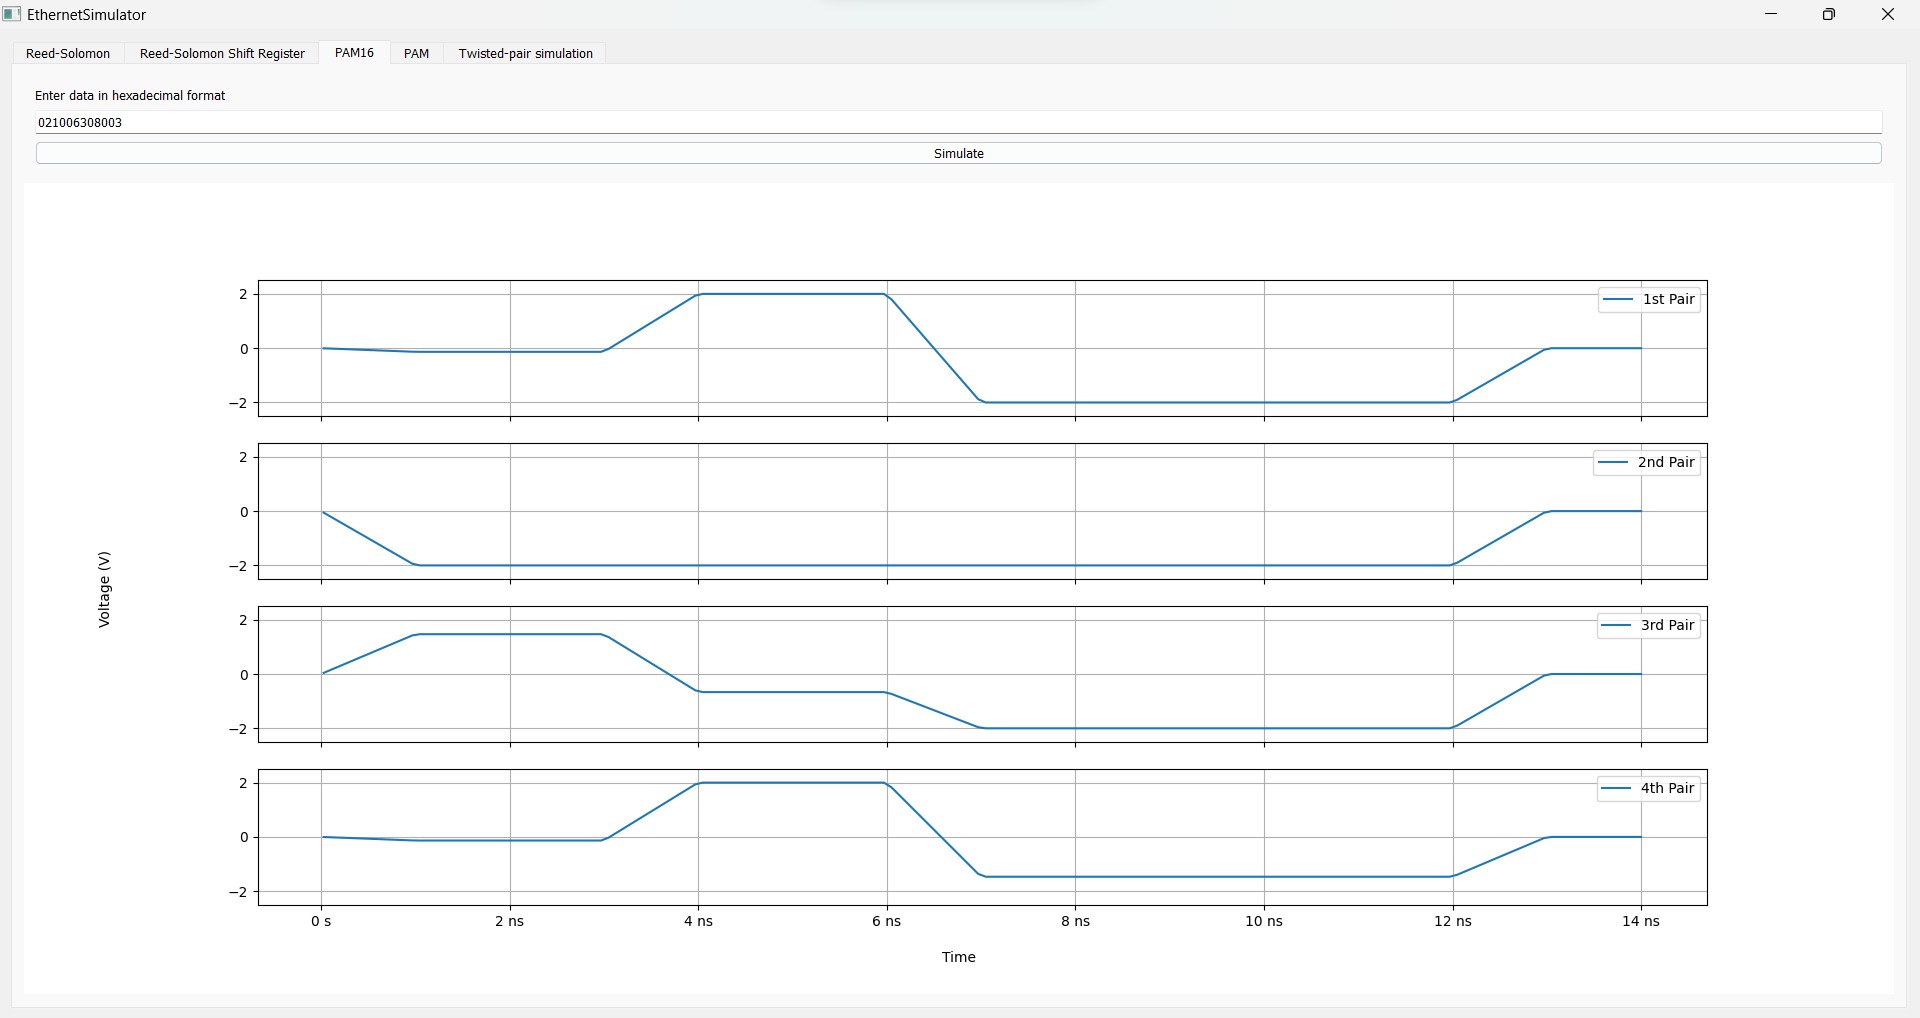
\includegraphics[width=0.95\textwidth, height=0.85\textheight,keepaspectratio]{prezentacja_pam16.png}
    \end{center}
\end{frame}

\begin{frame}
    \frametitle{PAM}
    \begin{center}
        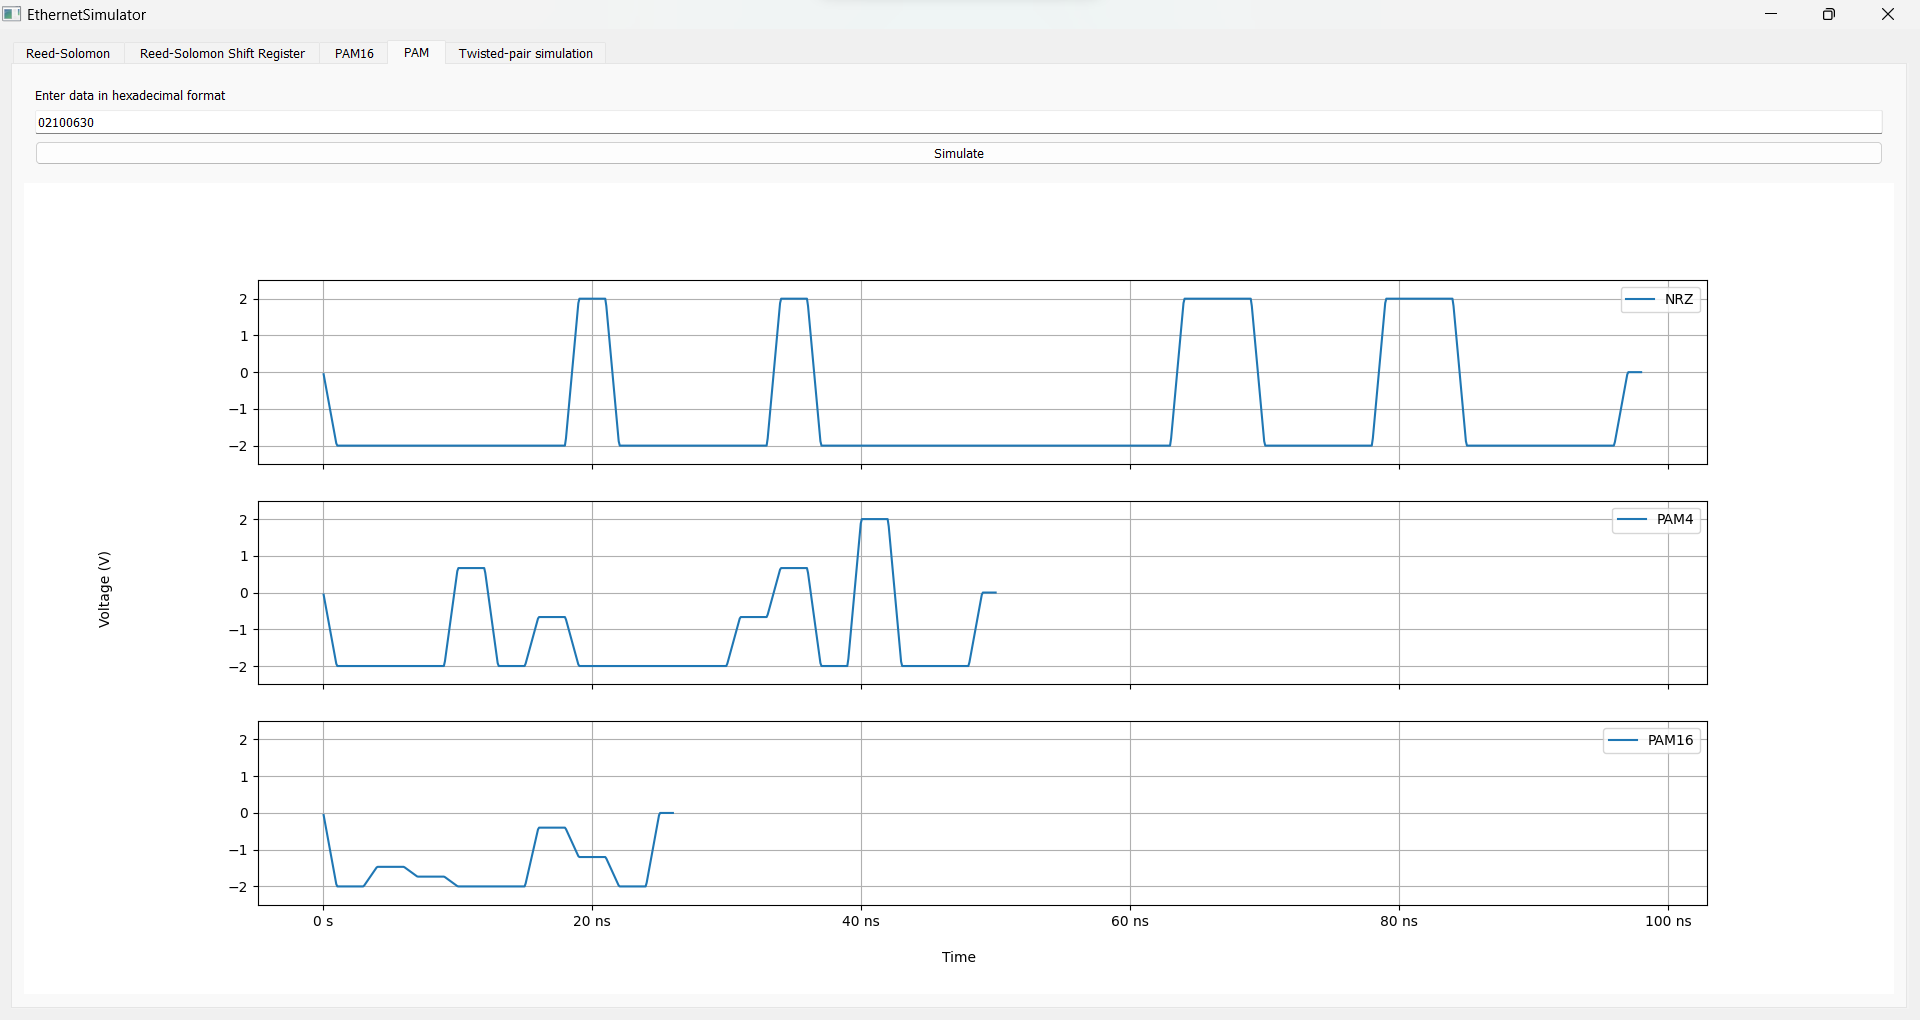
\includegraphics[width=0.95\textwidth, height=0.85\textheight,keepaspectratio]{prezentacja_pam.png}
    \end{center}
\end{frame}

\begin{frame}
    \frametitle{Twisted-pair simulation}
    \begin{center}
        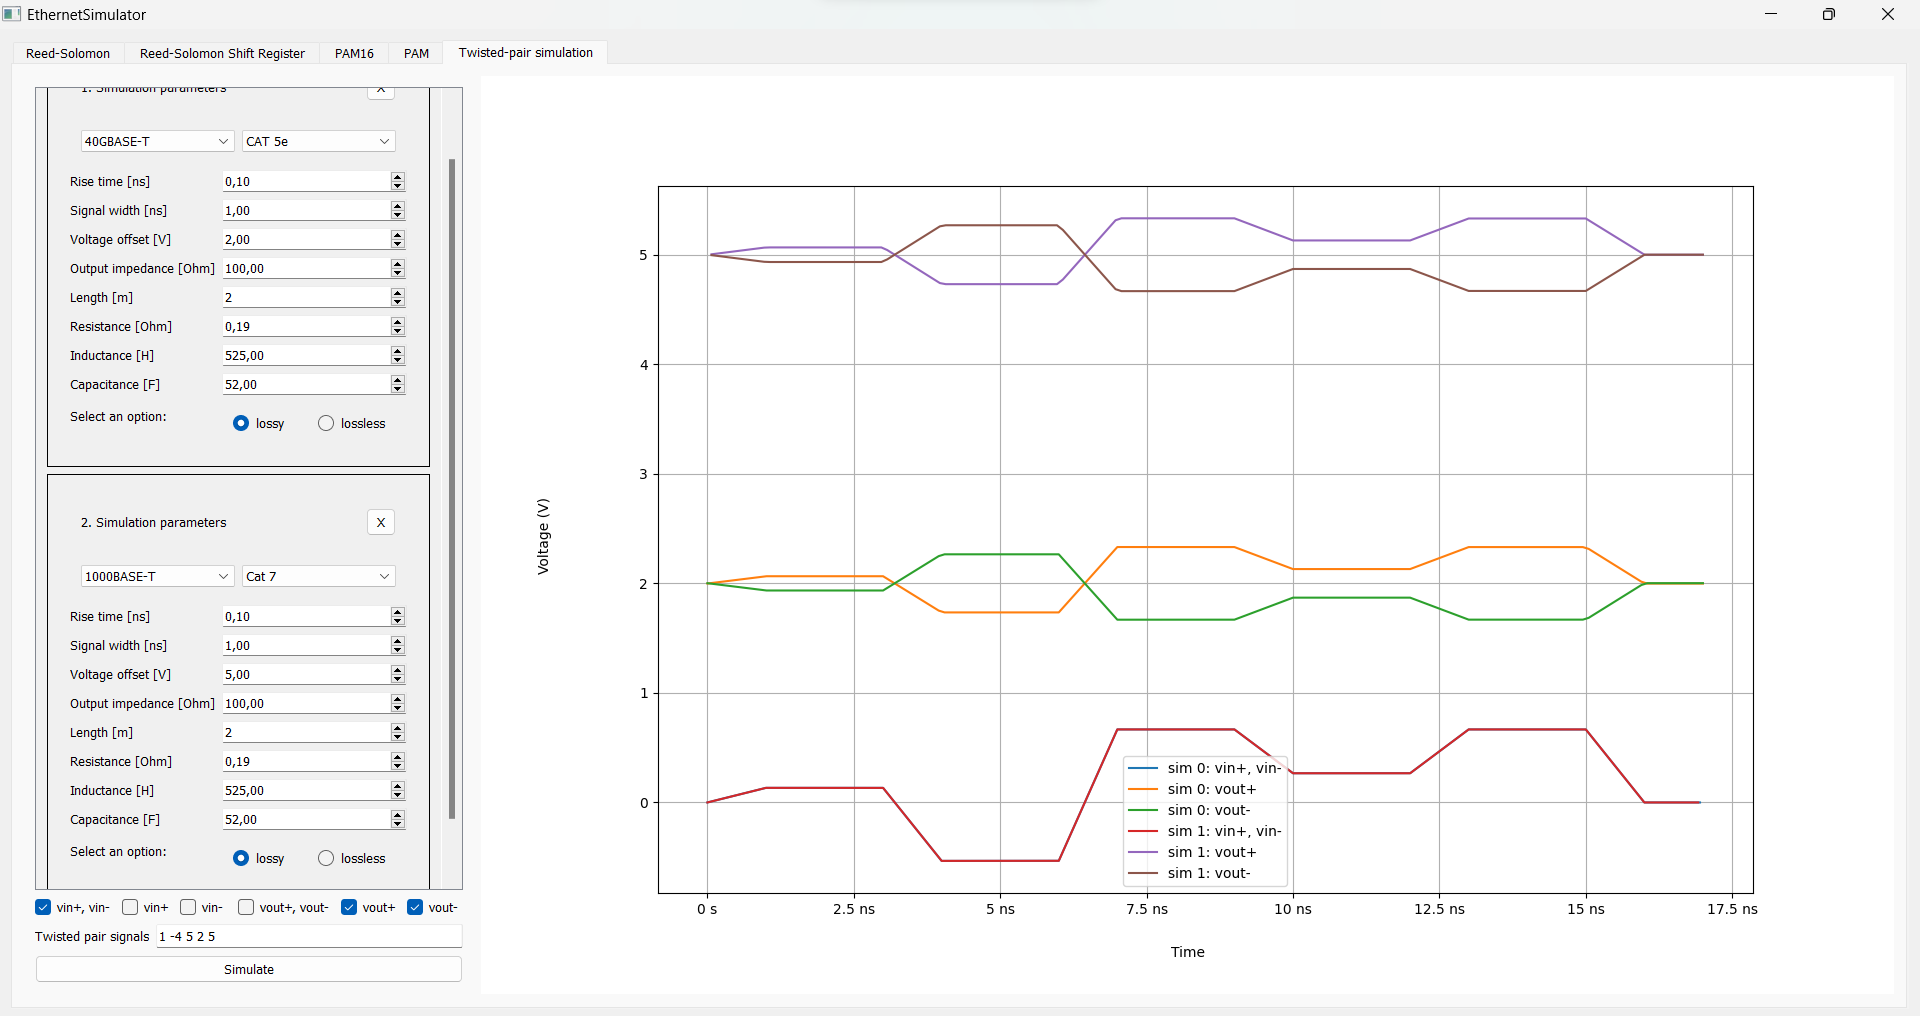
\includegraphics[width=0.95\textwidth, height=0.85\textheight,keepaspectratio]{prezentacja_tp.png}
    \end{center}
\end{frame}


% ------------------ REED SOLOMON -------------------------

\begin{frame}{Reed-Solomon}
	\begin{exampleblock}{Kod Reeda-Solomona}
		Kodowanie korekcyjne Reeda-Solomona zostało stworzone przez Irvina S. Reeda	oraz Gustava Solomona w 1960 roku.

		Kody Reeda-Solomona charakteryzują się kilkoma parametrami:

		\begin{itemize}
			\item Ciałem skończonym $\mathbb{F}_{q}$,  $q=2^m$, $m \in \{ 2, 3, \ldots \}$ w którym wykonywane są działania.
			\item długością wiadomości do zakodowania $k$
			\item długością słowa kodowego $n$ gdzie $k < n \leq q$
		\end{itemize}
	\end{exampleblock}
\end{frame}

\begin{frame}{Reed-Solomon}
	\begin{exampleblock}{Przykładowe kodowania RS(n,k,$\mathbb{F}_{2^m}$)
		w różnych standardach}
		\begingroup
			\hyphenpenalty10000
			\exhyphenpenalty10000
			\begin{table}[h]
			\centering
				\begin{tabular}{c p{6cm}}
				\toprule
				Kodowanie RS & Standardy \\
				\midrule
				RS(544, 514, $\mathbb{F}_{2^{10}}$)  & 50GBASE-R, 100GBASE-KP4, 200GBASE-R, 400GBASE-R \\
				\midrule
				RS(528, 514, $\mathbb{F}_{2^{10}}$) & 10GBASE-R, 25GBASE-R, 100GBASE-CR4 \\
				\midrule
				RS(450, 406, $\mathbb{F}_{2^9}$)  & 1000BASE-T1 \\
				\midrule
				RS(360, 326, $\mathbb{F}_{2^{10}}$)  & 2.5GBASE-T1, 5GBASE-T1, 10GBASE-T1 \\
				\midrule
				RS(192, 186, $\mathbb{F}_{2^8}$)  & 25GBASE-T, 40GBASE-T \\
				\bottomrule
				\end{tabular}
			\end{table}
		\endgroup
	\end{exampleblock}
\end{frame}

\begin{frame}{Warstwy Ethernet}
	\begin{center}
        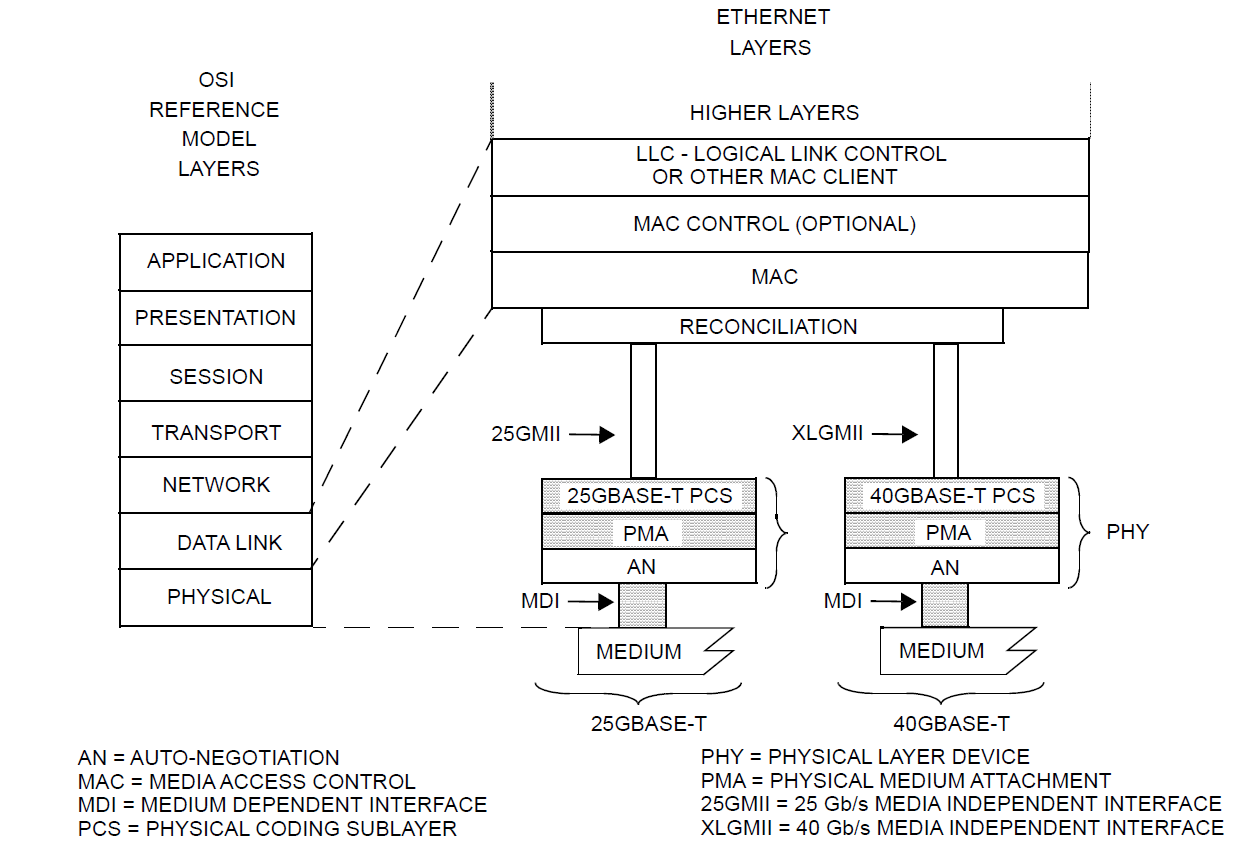
\includegraphics[width=0.95\textwidth,height=0.85\textheight,keepaspectratio]{25-40-gbase-osi.png}
    \end{center}
\end{frame}

\begin{frame}{25/40GBASE-T PCS}
	\begin{center}
        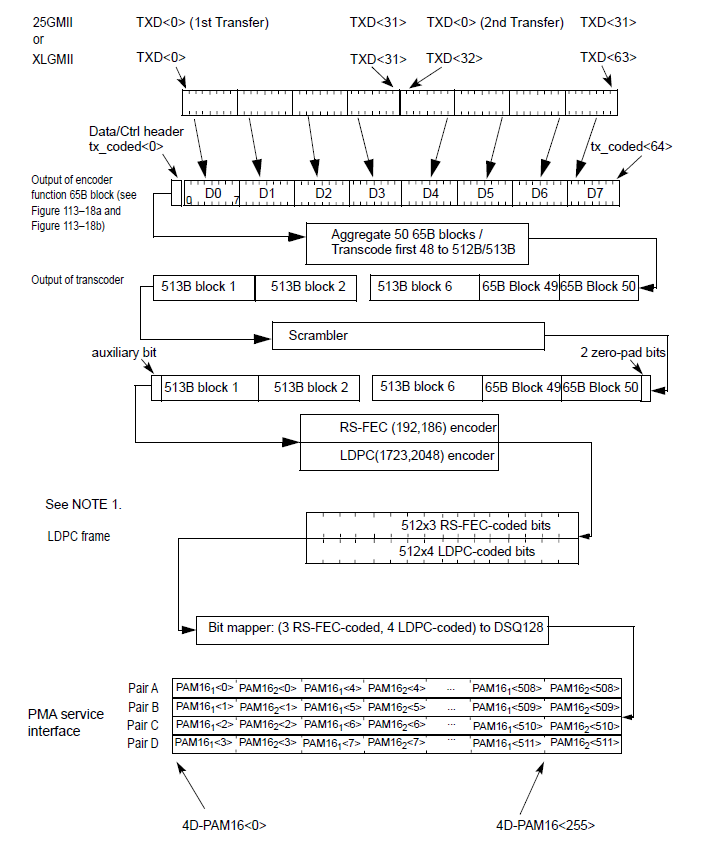
\includegraphics[width=0.95\textwidth,height=0.85\textheight,keepaspectratio]{25-40GBASE-T-coding.png}
    \end{center}
\end{frame}

\begin{frame}{2.5/5/10GBASE-T1 RS Encoder}
	\begin{center}
        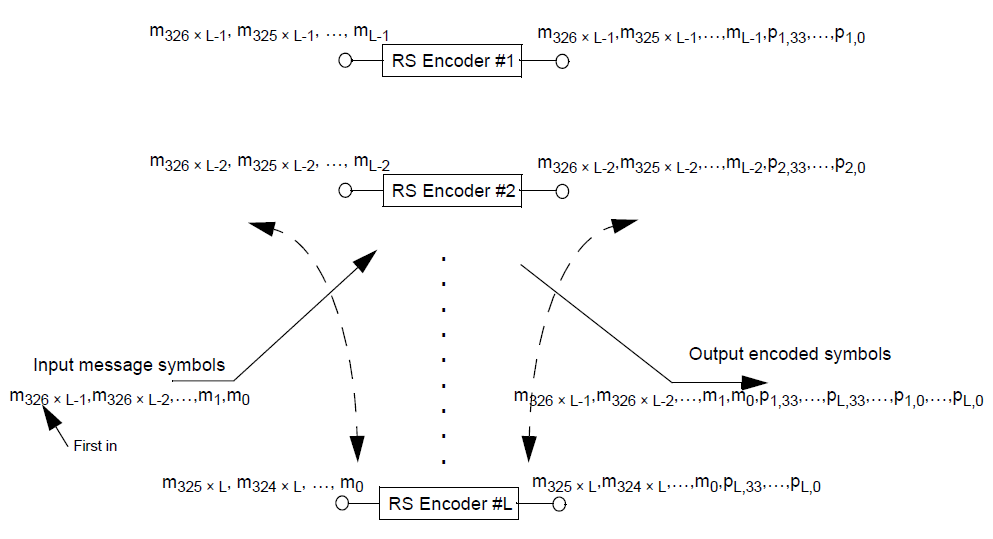
\includegraphics[width=0.95\textwidth,height=0.85\textheight,keepaspectratio]{rs-interleaver.png}
    \end{center}
\end{frame}

%------------------------------------------------

\subsection{Czym jest ciało}

\begin{frame}
	\frametitle{Czym jest ciało}

	Ciało $K$ jest to struktura algebraiczna $(K, +, \cdot, 0, 1)$ definiująca
	działania $+$ i $\cdot$ nazywane dodawaniem i mnożeniem.
	Działania te muszą spełniać kilka warunków:
	\begin{itemize}
		\item dodawanie i mnożenie jest łączne, przemienne oraz zawiera elementy neutralne
		\item każdy element musi posiadać element odwrotny względem dodawania
		\item każdy element oprócz $0$ musi posiadać element odwrotny względem mnożenia
		\item mnożenie jest rozdzielne względem dodawania
	\end{itemize}

\end{frame}

\subsection{Definicja ciała}

\begin{frame}
	\frametitle{Definicja ciała}

	Formalnie ciało (K, +, $\cdot$, 0, 1) definiuje się za pomocą kilku aksjomatów.
    \begin{exampleblock}{Aksjomaty ciała}
        \begin{align}
            a + (b + c) &= (a + b) + c & \forall a,b,c &\in K \\
            a \cdot (b \cdot c) &= (a \cdot b) \cdot c & \forall a,b,c &\in K \\
            a + b &= b + a & \forall a,b &\in K \\
            a \cdot b &= b \cdot a & \forall a,b &\in K \\
            a + 0 &= a & \forall a &\in K \\
            a \cdot 1 &= a & \forall a &\in K \\
            a + (-a) &= 0 & \forall a &\in K \: \exists {-a} \in K \\
            a \cdot a^{-1} &= 1 & \forall a &\in K \setminus \{ 0 \} \: \exists a^{-1} \in K \\
            a \cdot (b + c) &= (a \cdot b) + (a \cdot c) & \forall a,b,c &\in K
        \end{align}
    \end{exampleblock}
\end{frame}

\begin{frame}
	\frametitle{Ciało skończone}
    \begin{exampleblock}{Czym jest ciało skończone}
        Ciało skończone to po prostu ciało o skończonej liczbie elementów.
        Oznaczane jest zwykle jako $\mathbb{F}_q$ gdzie $q$ to liczba elementów.
        Aby ciało skończone istniało $q$ musi być liczbą pierwszą $p$ bądź potęgą
        takiej liczby $q=p^m$, $m \in \{ 2, 3, \ldots \}$
    \end{exampleblock}
\end{frame}

\subsection{Definicja ciała skończonego}
\begin{frame}
	\frametitle{Definicja ciała skończonego}

	Najprościej ciało skończone $\mathbb{F}_p$ gdzie $p$ to liczba pierwsza
	można zdefiniować jako pierścień klas reszt $\modulo{p}$.
	\begin{exampleblock}{Definicja tego pierścienia}
        \begin{align*}
            \modulo{p} &= \{ [0]_p, [1]_p, [2]_p, \ldots, [p-1]_p \} \\
            [a]_p &= \{ a + k \cdot p | k \in \mathbb{Z} \} \\
            \notag \\
            [a]_p + [b]_p &= [a + b]_p \\
            [a]_p \cdot [b]_p &= [a \cdot b]_p
        \end{align*}
    \end{exampleblock}
\end{frame}

\subsection{Charakterystyka ciała}

\begin{frame}
	\frametitle{Ciało skończone $\mathbb{F}_2$}
	Jednym z najczęściej używanych ciał skończonych w informatyce jest ciało
	$\mathbb{F}_2$ zawierające 2 elementy $\{ 0, 1 \}$ w którym działania $+$ i
	$\cdot$ są równoważne operacjom logicznym XOR oraz AND
    \begin{exampleblock}{Dodawanie i mnożenie w $\mathbb{F}_2$}
        \begin{table}
            \begin{tabular}{c c | c c}
                \toprule
                a & b & $+$ & $\cdot$ \\
                \midrule
                0 & 0 & 0 & 0 \\
                \midrule
                0 & 1 & 1 & 0 \\
                \midrule
                1 & 0 & 1 & 0 \\
                \midrule
                1 & 1 & 0 & 1 \\
                \bottomrule
            \end{tabular}
        \end{table}
    \end{exampleblock}
\end{frame}

\subsection{Ciało skończone \texorpdfstring{$\mathbb{F}_{2^m}$}{F\_2**m}}

\begin{frame}
	\frametitle{Ciało skończone $\mathbb{F}_{2^m}$}
	Elementami ciała skończonego $\mathbb{F}_{2^m}$,  $m \in \{ 2,3, \ldots \}$ są wielomiany o postaci
	\begin{align*}
		\sum_{n=0}^{m-1} c_n \alpha^n = c_{0} + c_{1}\alpha + c_{2}\alpha^{2} + \cdots + c_{m-1}\alpha^{m-1},
		c_{n} \in \{ 0, 1 \}
	\end{align*}
	\begin{exampleblock}{Przykładowe elementy $\mathbb{F}_{2^3}$}
		\begin{align*}
				\mathbb{F}_{2^3} &= \{ 0, 1, \alpha, \alpha + 1, \alpha^2, \alpha^2 + 1, \alpha^2 + \alpha, \alpha^2 + \alpha + 1 \} \\
				\mathbb{F}_{2^3} &= \{ 000_2, 001_2, 010_2, 011_2, 100_2, 101_2, 110_2, 111_2 \} \\
				\mathbb{F}_{2^3} &= \{ 0, 1, 2, 3, 4, 5, 6, 7 \}
		\end{align*}
	\end{exampleblock}
\end{frame}

\begin{frame}
	\frametitle{Dodawanie w $\mathbb{F}_{2^m}$}
	Dodawanie dwóch elementów ciała $\mathbb{F}_{2^m}$ jest po prostu obliczeniem XOR z ich reprezentacji binarnej

	\begin{exampleblock}{Przykład dodawania w $\mathbb{F}_{2^3}$}
		\begin{equation*}
			\begin{aligned}[t]
				a &= \alpha^2 + \alpha = 110_2 \\
				b &= \alpha + 1 = 011_2 \\
				a + b &= 110_2 \oplus 011_2
			\end{aligned}
			\qquad\qquad
			\begin{aligned}[t]
				&110_2 \\
				\oplus \; &011_2 \\
				\midrule
				&101_2
			\end{aligned}
		\end{equation*}
	\end{exampleblock}
\end{frame}

\begin{frame}
	\frametitle{Mnożenie w $\mathbb{F}_{2^m}$}
	Aby zdefiniować mnożenie w $\mathbb{F}_{2^m}$ potrzebujemy najpierw znaleźć
	nierozkładalny wielomian $p(x)$ stopnia	$m$ o współczynnikach w $\mathbb{F}_p$.
	Wynikiem mnożenia elementów ciała $\mathbb{F}_{2^m}$ będzie reszta z dzielenia
	iloczynu tych elementów przez wielomian $p(x)$

	\begin{exampleblock}{Przykład mnożenia w $\mathbb{F}_{2^3}$}
		\begin{align*}
			p(x) &= x^3 + x + 1 \\
			a &= \alpha^2 + 1 \\
			b &= \alpha + 1 \\
			a \cdot b &= (\alpha^2 + 1) \cdot(\alpha + 1) &\mod x^3 + x + 1 \\
			a \cdot b &= \alpha^3 + \alpha^2 + \alpha + 1 &\mod x^3 + x + 1 \\
			a \cdot b &= \alpha^2
		\end{align*}
	\end{exampleblock}
\end{frame}

\begin{frame}
	\frametitle{Mnożenie w $\mathbb{F}_{2^m}$}
	\begin{exampleblock}{Reszta z dzielenia przez $p(x)$}
		$a \cdot b = \alpha^3 + \alpha^2 + \alpha + 1 = 1111_2$
		\newline
		$p(x) = x^3 + x + 1 = 1011_2$
		\begin{equation*}
			\begin{split}
				          &1 \\
						  \toprule
				          &1111 : 1011 \\
				\oplus \; &1011 \\
						  \midrule
						  &\;100 = \alpha^2
			\end{split}
		\end{equation*}
	\end{exampleblock}
\end{frame}

\begin{frame}
	\frametitle{Reed-Solomon}
	\begin{exampleblock}{Właściwości}
		Kody Reeda-Solomona cechują się możliwością korekty $\lfloor \frac{n-k}{2} \rfloor$
		lub wykrycia $n-k$ błędnych symboli. Symbol w ciele $\mathbb{F}_{2^m}$ składa się
		z $m$ bitów co w przypadku błędów grupowych daje możliwość korekty maksymalnie
		$m \cdot \lfloor \frac{n-k}{2} \rfloor$ bitów bądź detekcji $m(n-k)$ przekłamanych
		bitów
	\end{exampleblock}
\end{frame}

\begin{frame}
	\frametitle{Reed-Solomon}
	\begin{exampleblock}{Oryginalny sposób kodowania}
		Sposób kodowania przedstawiony w pracy Reeda i Solomona polega na stworzeniu
		wielomianu $p_m(x)=\sum_{i=0}^{k-1}m_{i}x^i$, gdzie $m_i\in\mathbb{F}_q$ to
		$i$\nobreakdash-ty element wiadomości, po czym za pomocą tego wielomianu
		obliczane jest słowo kodowe $C(m)=(p_m(a_0), p_m(a_1), \ldots, p_m(a_{n-1}))$
		gdzie $a_i$ to różne elementy ciała $\mathbb{F}_q$.
	\end{exampleblock}
\end{frame}

\begin{frame}
	\frametitle{Reed-Solomon}
	\begin{exampleblock}{Kod systematyczny}
		Za pomocą niewielkiej modyfikacji można stworzyć kod systematyczny czyli taki w którym słowo kodowe zawiera w sobie kodowaną wiadomość.
		Żeby stworzyć kod systematyczny musimy zmodyfikować sposób tworzenia wielomianu w taki sposób by $p_m(x_i)=m_i$ dla $i \in \{0,1,\ldots,k-1\}$.

		Jednym ze sposobów stworzenia takiego wielomianu jest użycie metody interpolacji wielomianów. Słowo kodowe wygenerowane z tego wielomianu będzie zawierało wiadomość w pierwszych $k$ elementach.
		\begin{align*}
			C(m) &= (p_m(a_0), p_m(a_1), \ldots, p_m(a_{n-1})) \\
			&=(m_0, m_1, \ldots, m_{k-1}, p_m(a_k), p_m(a_{k+1}), \ldots, p_m(a_{n-1}))
		\end{align*}
	\end{exampleblock}
\end{frame}

\begin{frame}
	\frametitle{Reed-Solomon}
	\begin{exampleblock}{Kod BCH}
		Kody BCH~(Bose-Chaudhuri-Hocquenghem) są kodami cyklicznymi co oznacza że
		każde przesunięcie słowa kodowego jest także słowem kodowym.

		Aby zbudować kod BCH Reeda-Solomona potrzebujemy najpierw funkcji minimalnej
		pierwiastka $\alpha$, czyli takiego minimalnego wielomianu nierozkładalnego
		$p(x)$ stopnia $m$ dla którego istnieje element prymitywny $\alpha$ który pozwala wygenerować całe ciało skończone
		\begin{align*}
			\mathbb{F}_{2^m} = \{0, 1, \alpha, \alpha^2, \ldots, \alpha^{p^{m}-1} \}
		\end{align*}
	\end{exampleblock}
\end{frame}

\begin{frame}
	\frametitle{Reed-Solomon}
	\begin{exampleblock}{Obliczanie kodu BCH}
		Mając taki element prymitywny jesteśmy w stanie stworzyć wielomian generujący $g(x)$ używając wzoru
		\begin{align*}
			t &= n - k \\
			g(x) = \prod_{i=0}^{t-1} (x - \alpha^i) &= g_{t}x^t + g_{t-1}x^{t-1} +
			\cdots + g_{1}x + g_{0}
		\end{align*}
		Aby utworzyć słowo kodowe wystarczy pomnożyć wielomian $p_m(x)$ przez wielomian generujący $g(x)$

		Aby uzyskać systematyczne słowo kodowe $s(x)$ musimy obliczyć:
		\begin{align*}
			s_r(x) &= p_m(x) \cdot x^t \mod g(x) \\
			s(x) &= p_m(x) \cdot x^t - s_r(x)
		\end{align*}
	\end{exampleblock}
\end{frame}

\end{document}
